\documentclass[brazil,ruledheader]{abntifes}
%\documentclass[brazil,twoside,ruledheader]{abntifes}
\usepackage[T1]{fontenc}
%\usepackage[latin1]{inputenc}
\usepackage[utf8]{inputenc}
\usepackage[brazil]{babel}
\usepackage[]{algorithm2e}
\usepackage{pslatex}
\usepackage{url}
\usepackage{fancyhdr}
\usepackage{graphicx}
\usepackage{amsmath, amsthm, amssymb}
\usepackage{exercise}
\usepackage{makeidx}
\usepackage{setspace}
\usepackage{multicol}
\usepackage{upquote}
\usepackage{graphicx}
\usepackage{float}
\usepackage{epigraph}

\usepackage{listings,xcolor}

% Define o caminho das figuras
\graphicspath{{capitulos/figuras/}}

\definecolor{dkgreen}{rgb}{0,.6,0}
\definecolor{dkblue}{rgb}{0,0,.6}
\definecolor{dkyellow}{cmyk}{0,0,.8,.3}
\lstset{
  language         = PHP,
  extendedchars = \true,
  keepspaces = true,
  basicstyle       = \small\ttfamily,
  % upquote          =true,
  % numbers          =left,
  stepnumber       =1,
  numbersep        =10pt,
  showstringspaces =false,
  breaklines       =true,
  frameround       =ftff,
  frame            =single,
  belowcaptionskip =5em,
  belowskip        =3em,
  numberstyle      =\tiny\color{gray},
  keywordstyle     = \color{dkblue},
  stringstyle      = \color{red},
  identifierstyle  = \color{dkgreen},
  commentstyle     = \color{gray},
  emph             =[1]{php},
  emphstyle        =[1]\color{black},
  emph             =[2]{if,and,or,else},
  emphstyle        =[2]\color{dkyellow}
  keywordstyle = \bfseries,
  morekeywords={function,return}
}


% \lstset{language=PHP,
%     commentstyle = \color{gray},
%     inputencoding = utf8x,
% }
% \lstset{numbers=left, stepnumber=5, firstnumber=1, numberstyle=\tiny, extendedchars=true, breaklines=true, frame=tb, basicstyle=\footnotesize, stringstyle=\ttfamily, showstringspaces=false }

%\makenomenclature

% Para listar programas em C#
% \lstdefinelanguage{cs}
%   {morekeywords={abstract,event,new,struct,as,explicit,null,switch
% 		base,extern,object,this,bool,false,operator,throw,
% 		break,finally,out,true,byte,fixed,override,try,
% 		case,float,params,typeof,catch,for,private,uint,
% 		char,foreach,protected,ulong,checked,goto,public,unchecked,
% 		class,if,readonly,unsafe,const,implicit,ref,ushort,
% 		continue,in,return,using,decimal,int,sbyte,virtual,
% 		default,interface,sealed,volatile,delegate,internal,short,void,
% 		do,is,sizeof,while,double,lock,stackalloc,
% 		else,long,static,enum,namespace,string, },
% 	  sensitive=false,
% 	  morecomment=[l]{//},
% 	  morecomment=[s]{/*}{*/},
% 	  morestring=[b]",
% }

\newcommand{\AUTOR}{Guilherme Peixoto da Costa Louro}
\newcommand{\SEGUNDOAUTOR}{}
\newcommand{\ORIENTADOR}{Maria do Carmo Facó}
\newcommand{\COORIENTADOR}{}
\newcommand{\TITULO}{Desenvolvimento do Framework Lothus\{PHP\}}
\newcommand{\CURSO}{Tecnólogo em Tecnologia da Informação e da Comunicação}
\newcommand{\GRAU}{Tecnólogo em Tecnologia da Informação e da Comunicação}
% \newcommand{\GRAU}{Tecnólogo em Análise e Desenvolvimento de Sistemas}
\newcommand{\INSTITUICAO}{Faculdade de Educação Tecnológica do Estado do Rio de Janeiro Faeterj/Petrópolis}
\newcommand{\ANO}{Julho, 2015}
\newcommand{\DATA}{31 de Julho de 2015}
\newcommand{\LOCAL}{Petrópolis - RJ}
\newcommand{\epigrafe}{\vspace{1cm}{\raggedright\par\sffamily\slshape\par}}
\begin{document}

\autor{\AUTOR}
\titulo{\TITULO}
\orientador{\ORIENTADOR}
\coorientador{\COORIENTADOR}

\comentario{Trabalho de Conclusão de Curso apresentado à Coordenadoria do Curso de \CURSO\
	    da \INSTITUICAO , como requisito parcial para obtenção do título de \GRAU .}

\instituicao{\INSTITUICAO}
\curso{\CURSO}
\governo{Governo do Estado do Rio de Janeiro}
\secretaria{Secretaria de Estado de Ciência e Tecnologia}
\fundacao{Fundação de Apoio à Escola Técnica}
\cpti{Centro de Educação Profissional em Tecnologia da Informação}
\local{\LOCAL}
\data{\ANO}

\capa

\folhaderosto

% Ficha Catalográfica
%\begin{figure}
%\includegraphics[width=11cm]{FichaCatalografica.pdf}
%\end{figure}

% Folha de Aprovação
\newpage
\vfill
\null
\begin{center}
{\Huge {\bfseries\itshape Folha de Aprovação}}\\[3cm]
\begin{espacoduplo}
Trabalho de Conclusão de Curso sob o título \textit{``\TITULO''},
defendida por \AUTOR\ e aprovada em \DATA, em \LOCAL, pela banca examinadora constituída pelos
professores: \setlength{\ABNTsignthickness}{0.4pt}
\end{espacoduplo}
\setlength{\ABNTsignthickness}{0.4pt}

% ou inserir a página assinada e escaneada aqui
%\begin{figure}
%\includegraphics[]{Fo	lhaAprovacao.pdf}
%\end{figure}


\assinatura{Prof. \ORIENTADOR\\ Orientador}
\assinatura{Prof. Banca Interna \\ \INSTITUICAO}
\assinatura{Prof. Banca Interna \\ \INSTITUICAO}
%\assinatura{Prof. Banca Externa \\ Instituto do membro externo}

\end{center}


% Folha do Termo de Compromisso
\newpage

\vfill
\null
\begin{center}
{\Huge {\bfseries\itshape Declaração de Autor}}\\[3cm]
\begin{espacoduplo}
Declaro, para fins de pesquisa acadêmica, didática e tecnico-científica, que o presente Trabalho de Conclusão
de Curso pode ser parcial ou totalmente utilizado desde que se faça referência à fonte e aos autores.
\end{espacoduplo}
\setlength{\ABNTsignthickness}{0.4pt}
\assinatura{\AUTOR}
Petrópolis, em \DATA
\end{center}



\chapter*{Dedicatória}
    Dedico esse trabalho a membros de minha família e amigos, principalmente a minha noiva por estar ao meu lado a todo momento me apoiando, mesmo nos momentos mais difíceis, nessa caminhada de dois anos e meio de faculdade e mais dois anos entre a criação do projeto e algumas pausas por motivos pessoais.

    Gostaria de agradecer também aos que foram importantes em minha vida, me apoiando e motivando desde a escolha da faculdade até seus momentos finais.

    Não podendo deixar de dedicar o trabalho aos companheiros de classe que viveram comigo os momentos fáceis e os mais complicados de toda a trajetória do curso, sem esquecer os que, de algum lugar, me mandou energia e motivação para a conclusão deste trabalho.


\chapter*{Agradecimentos}
    Ao meu orientador, professores e companheiros de trabalhor que se envolveram no desenvolvimento deste trabalho e deste projeto. Em especial agradeço a minha família e a minha noiva pela motivação e compreensão em momento dificeis e de ausência de minha parte em resultado à dedicação dada a este projeto.
\vfill
\null

\begin{center}
{\Huge {\bfseries\itshape Epígrafe}}\\[3cm]
\vspace{15cm}
\end{center}

\begin{espacoduplo}
\end{espacoduplo}

% Não é obrigadorio ter epigrafe
\epigraph{"Frase de efeito"}{(Autor)}

\begin{resumo}
    O mercado atual proporciona ao desenvolvedor diversas ferramentas, capazes de possibilitar a criação de sistemas de forma ágil e automatizada. Contudo, ferramentas como essas, dependem de um estudo baseado em suas documentações a fim de se produzir um sistema de forma correta, sem fugir das determinações exigidas pela ferramenta utilizada. Esse processo, na maioria dos casos, exigem um certo tempo para o entendimento de todas as funcionalidades e métodos possíveis de serem usados, fazendo com que alguns desenvenvolvedores acabe testando outras ferramentas sem se especializar em nenhuma delas.

    A proposta do projeto, apresentado neste documento, é de um framework capaz de suprir as necessidades mais importantes no desenvolvimento de um site ou sistema web. De forma simples e sem a complexidade de ferramentas que já existem no mercado, o \emph{Framework Lothus\{PHP\}} busca atender todos os niveis de desenvolvedores, principalmente por ter uma curta curva de aprendizagem.

    O \emph{Framework Lothus\{PHP\}} utiliza MVC \emph{(Model, View, Controller)} como padrão de projetos e foi produzido de forma à atender desenvolvedores FrontEnd e BackEnd, trazendo uma estrutura de pastas que separa cada etapa do processo de desenvolvimento.

    Será detalhado todo o processo de desenvolvimento do \emph{Framework}, mostrando todas as diretrizes e funcionalidades de cada etapa da criação do mesmo. Este detalhamente será apresentado com explicações sobre arquivos e trechos de códigos pertencentes ao \emph{Framework}, passando de forma transparente o funcionamento de cada etapa.

    Ao detalhar todo o processo de criação do \emph{Lothus \{PHP\}}, será descrito todas as ferramentas e tecnologias usadas para auxiliar o desenvolvimento capaz de tornar ágil futuras aplicações produzidas através do \emph{Framework}.

    Por fim será apresentado a criação de um pequeno projeto usando algumas técnicas do \emph{Framework Lothus\{PHP\}} através de um passo-a-passo capaz de deixar claro o quanto ele pode agilizar o processo de desenvolvimento de uma forma facil e equilibrada. Além disso será apresentado alguns sistemas feitos usando o \emph{Framework}.
\end{resumo}


\begin{abstract}
Resumo em inglês ... "Não é obrigadorio"
\end{abstract}

\listoffigures

\listoftables

%Lista de abreviaturas

\tableofcontents{}


% Capitulo 1
\chapter{Introdução\label{cap:introducao}}
    Devido à grande necessidade de entregar projetos de grande porte e com prazos consideravelmente baixos, foi percebida a necessidade de se encontrarem soluções que facilitassem esse desenvolvimento.

    A primeira atitude a ser tomada foi a criação de um arquivo que reunisse diversas funcionalidades, a fim de facilitar futuros projetos, onde processos que se repetiam diversas vezes eram colocados em funções que poderiam ser usadas em novos projetos.

    Aplicações, em geral, precisam de um padrão mais significativo como forma estrutural de um projeto, deixando claro que a criação de um arquivo contendo todas as funções do projeto não era o melhor padrão a ser seguido. Este trabalho apresenta, como uma de suas justificativas, uma pesquisa profunda que reúne novos padrões para os processos e \emph{Frameworks} web que poderiam ser mais úteis para um desenvolvimento ágil.

    No final dessas pesquisas iniciais, alguns \emph{Frameworks} foram testados e o CakePHP passou a ser usado como padrão. O CakePHP utiliza o padrão de projeto MVC \emph{(Model, View, Controller)} que é um modelo de arquitetura de software que tem como objetivo básico separar a lógica de negócio da aplicação.

    Os \emph{Frameworks} são sempre muito robustos e com diversos tipos de funcionalidades, e com o CakePHP não é diferente. Com uma vasta documentação e uma quantidade considerável de arquivos em seu projeto mais simples, este passou a ser um problema ao invés de solução quando se busca um total domínio em uma aplicação.

    Percebeu-se, então, a real necessidade de criar um Framework onde se tenha total controle de todas as funcionalidades, mantendo o padrão MVC, porém criando as próprias funcionalidades, mesmo que baseado em funcionalidades de outros \emph{Frameworks}.

    Identificar o problema foi o primeiro e principal passo para se iniciar o desenvolvimento do \emph{Framework}, que se encontra sempre em evolução com novas implementações que resolvam determinados problemas.


% Capitulo 2
\chapter{A import\^ancia de se usar Framework\label{cap:importancia}}
    Neste capítulo será apresentado, com dados técnicos, a importância do uso de um \emph{Framework} em projetos de desenvolvimento, detalhando algumas de suas vantagens e desvantagens no processo de codificação.

    O \emph{framework} é, como princ\'ipio b\'asico, uma arquitetura "padrão" que tem como objetivo fornecer ferramentas comuns a todo tipo de projeto, utilizando os mais variados tipos de Design Pattern (Padrões de Projeto) a fim de proporcionar um ambiente de desenvolvimento extremamente produtivo.

    Grande parte dos \emph{Frameworks} trabalham com um padrão principal denominado MVC (Model View Controller) que tem como base trabalhar com Modelo Lógico (Model), onde acontece toda a interação com a base de dados do projeto, Visualização (View), que é a parte responsável pela exibição de dados, e o Controle (Controller), que é a regra de negócios do projeto, pode-se dizer que o Controller é responsável por fazendo toda a comunicação com o Model e tratar os dados para serem exibidos pela View. Resumindo, o padrão MVC separa claramente o Design do Conteúdo e de sua Lógica.

    \section{Vantagens em usar um Framework\label{sec:vantagens-framework}}
        \begin{itemize}
            \item \textbf{Padronização em projetos}: A grande vantagem de um \emph{framework} é sua padronização no desenvolvimento. Por utilizar um conjunto já definido de Classes e Métodos, a necessidade de trabalhar conforme a ferramenta possibilita ajudar a garantir um aproveitamento maior de código projetos futuros.

            \item \textbf{Velocidade no desenvolvimento}: O fato de se fazer uso de módulos genéricos faz com que o \emph{framework} fique responsável por controlar o uso de funcionalidades repetitivas fazendo com que o desenvolvedor se concentre totalmente na regra de negócios de cada projeto.

            \item \textbf{Qualidade}: \emph{Frameworks} em geral são testados e atualizados a todo momento, tornado-se cada vez mais seguros e com melhores funcionalidades.

            \item \textbf{Re-uso de códigos}: A padronização de projetos torna capaz o re-uso de código sem dificuldades de adaptação.

            \item \textbf{Segurança}: Uma das vantagens mais importantes é a segurança que o \emph{Framework} pode dar ao projeto.

            \item \textbf{Fácil manutenção}: A separação do \emph{framework}, utilizando padrões de projetos, permite uma fácil manutenção em determinada ferramenta sem que afete outras.

            \item \textbf{Utilitários e Bibliotecas}: Classes e métodos embutidos no \emph{framework} para solucionar o problema de repetição contínua de códigos.
        \end{itemize}

    \section{Desvantagens em usar um Framework\label{sec:desvantagens-framework}}
        Esses pontos não são necessariamente uma desvantagem, porém são os principais motivos que inibem o desenvolvedor de iniciar em um \emph{Framework}.

        \begin{itemize}
            \item \textbf{Performance e peso}: A grande quantidade de arquivo, a chamada de métodos e a criação de objetos nem sempre necessários para determinados projetos tornam a aplicação pesada em alguns casos.

            \item \textbf{Curva de aprendizado}: Ao se trabalhar com códigos de terceiros, existe uma curva de aprendizado elevada e que fica dependente de uma boa documentação para conseguir atingir um bom ritmo de trabalho.

            \item \textbf{Conhecimento técnico}: É necessário que se tenha conhecimento em OOP (Programação Orientada a Objeto), boas práticas de programação e se entendam padrões de projetos para poder utilizar o \emph{Framework} da melhor forma.

        \end{itemize}


% Capitulo 3
\chapter{Métodos e materiais\label{cap:metodos-materiais}}
    Com o intuito de apresentar todo o processo de criação e utilização das ferramentas e funcionalidades do \emph{Framework Lothus\{PHP\}}, neste capítulo serão apresentados e descritos os elementos e métodos utilizados para seu desenvolvimento e funcionamento.

    \section{PHP\label{sec:php}}
      O PHP (\emph{um acrônimo recursivo para PHP: Hypertext Preprocessor}) é uma linguagem de script open source de uso geral, muito utilizada, e especialmente adequada para o desenvolvimento web e que pode ser embutida dentro do HTML.i(Php.net,2015).

      O PHP contém um HTML com códigos embutidos que permite unir linguagem de marcação a códigos extremamente dinâmicos, utilizando as tags '\textbf{<?php}' e '\textbf{?>}' que separam o \emph{HTML} do \emph{PHP}.

      É uma linguagem server-side (\emph{lado do servidor}) e tem seu código executado diretamente no servidor, retornando somente o HTML que será exibido para o cliente, omitindo o acesso ao código PHP da aplicação.


    \section{POO \emph{(Programação Orientada a Objetos)}\label{sec:poo}}
        Programação Orientada a Objetos é um padrão de desenvolvimento com um conjunto de ideias, conceitos e princípios utilizados para facilitar e organizar melhor o desenvolvimento de aplicações. Tem como principais características facilitar a manutenção de códigos, utilizar com frequencia o reaproveitamento de códigos, além de diminiur a complexidade no desenvolvimento de sistemas.


        \subsection{Principais conceitos de POO\label{sub:principais-conceitos}}
            \begin{itemize}
                \item \textbf{Abstração}: Utilizada para a definição de entidades do mundo real.
                        \begin{figure}[!htb]
                            \centering
                            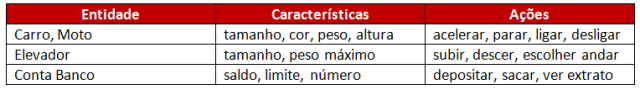
\includegraphics{abstracao.jpg}
                            \caption{\small Abstração do mundo real.}
                            \label{cap:conceitos}
                        \end{figure}
                \item \textbf{Classes}: Definição dada para a estrutura de um objeto, onde são definidas os atributos e métodos referentes a cada objeto.

                \item \textbf{Objetos}: É a instância de uma classe. Um objeto é a construção de software que encapsula estado e comportamento, nos permitindo modelar a aplicação em termos reais e abstrações.

                \item \textbf{Herança}: É a possibilidade de uma classe \emph{(subclasse)} herdar métodos e atributos de outra classe \emph{(superclasse)}
                        \begin{figure}[!htb]
                            \centering
                            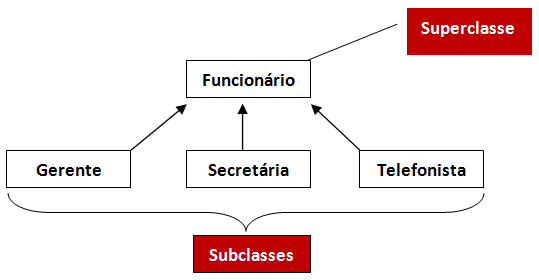
\includegraphics{heranca.jpg}
                            \caption{\small Hieraquia de classes}
                            \label{cap:heranca}
                        \end{figure}
                \item \textbf{Polimorfismo}: Se trata da capacidade de um método ou comportamento da \emph{superclasse} ser implementado de diversas maneiras nas \emph{subclasses}.
                \item \textbf{Encapsulamento}: Forma de proteção dos atributos de uma classe, não permitindo que este seja acessado diretamente.

            \end{itemize}


    \section{MVC \emph{(Model, View e Controller)} \label{sec:mvc}}
        O MVC é um Design Pattern \emph{(Padrão de projeto)} utilizado para separar as camadas de modelo, visão e controle no desenvolvimento de um sistema. A camada de modelo \emph{(Model)} contém classes que implementam a regra de negócios da aplicação. A camada de visão \emph{(View)}, por sua vez, é responsável pela exibição e apresentação dos dados para o usuário, e, por fim, a camada de controle \emph{(Controller)}, onde são processadas todas as requisições realizadas pelos usuários.

        A separação da aplicação em camadas, como é feita no padrão MVC, trás uma série de vantagens no processo de desenvolvimento: uma delas é a de permitir a reutilização do mesmo objeto de modelo em visualizações distintas, além de organizar seu projeto de forma onde tudo tenha seu lugar, e cada camada com sua responsabilidade, permitindo um trabalho muitos mais "centrado" e modularizado.


    \section{CRUD \emph{(Create, Read, Update e Delete)}\label{sec:crud}}
        CRUD é o acrônimo da expressão do idioma inglês, \emph{Create Read Update and Delete} e é utilizado para designar as quarto operaçõs básicas de um banco de dados: Criar, Ler, Atualizar e Deletar.
        \begin{figure}[!htb]
            \centering
            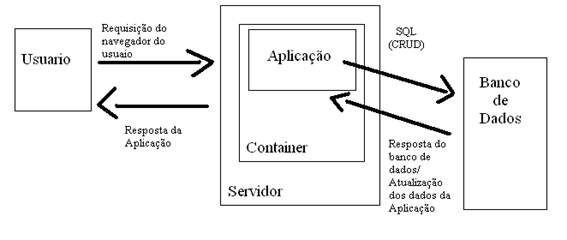
\includegraphics{crud.jpg}
            \caption{\small Execução de uma requisição CRUD}
            \label{cap:crud}
        \end{figure}

        Tratando como uma forma mais técnica, o CRUD se transforma em um facilitador, criado através de diretivas de programação, para ações ligadas ao \emph{INSERT}, \emph{UPDATE}, \emph{DELETE} e \emph{SELECT} do banco de dados.



    \section{UML\label{sec:uml}}
        UML \emph{(Unified Modeling Language)}, é uma linguagem de modelagem que possibilita o desenvolvimento de diagramas de classes, de objetos, casos de uso, entre outros. Esses diagramas são úteis para o desenvolvimento e um grande facilitador para o entendimento de um projeto e sua estrutura.

        \begin{figure}[!htb]
            \centering
            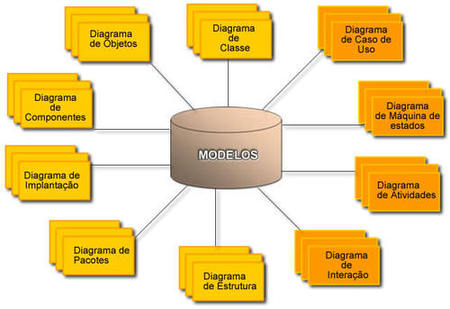
\includegraphics{uml.jpg}
            \caption{\small Exemplo de um diagrama UML.}
            \label{cap:uml}
        \end{figure}


    \section{Mysql\label{sec:mysql}}
        O MySQL é um gerenciador de banco de dados de código aberto, capaz de atender às necessidades dos mais variados tipos de usuários. Este produto tem uma gama diversificada de possibilidades de uso, algumas delas são soluções em desenvolvimento de sistemas, provedores, aplicações livres, entre outras.

    \section{PDO\label{sec:pdo}}
        PDO \emph{(PHP Data Objects)} é um módulo de PHP montado sob o paradigma Orientado a Objetos e cujo objetivo é prover uma padronização da forma com que PHP se comunica com um banco de dados relacional. Este módulo surgiu a partir da versão 5 de PHP. PDO, portanto, é uma interface que define um conjunto de classes e a assinatura dos métodos de comunicação com uma base de dados. (LOCAWEB, 2015)

    \section{HTML\label{sec:hmtl}}
        HTML \emph{(Hyper Text Markup Language)}, como o próprio nome já diz, é uma linguagem de marcação de hipertexto utilizada no desenvolvimento de páginas web. Ela nos possibilita estruturar uma página através de marcações e tags específicas, permitindo que a mesma seja acessada pela internet.

    \section{Node.js\label{sec:node-js}}
        \emph{Node.js} é uma plataforma construída sobre o motor de Javascript que tem como principal objetivo fornecer uma maneira fácil de se construir programas de rede escaláveis. Mesmo sendo um servidor de programas, não podemos confundi-lo com um servidor \emph{ready-to-install}(prontos para instalar), que são servidores que estão prontos para instalar aplicativos instantaneamente. O \emph{Node.js} segue o conceito de módulos que podem ser adicionados em seu núcleo. Há literalmente centenas de módulos para rodarem com o Node, e a comunidade é bastante ativa em produzir, publicar e atualizar dezenas de módulos por dia.

    \section{Automatizador Grunt\label{sec:automatizador-grunt}}
        \emph{Grunt} é uma ferramenta que roda via termina e serve para automatizar tarefas de uma aplicação,  como: concatenação, minificação e validação de arquivos, otimização de imagem, testes unitários, deploy de arquivos por ftp ou rsync, entre outras. O \emph{Grunt} é feito totalmente em \emph{Javascript} e roda no \emph{Node.js}, portanto para ser utilizado, depende da instalação do \emph{Node.js} e do pacote \emph{NPM} previamente instalados.

    \section{Sass\label{sec:sass}}
        É um pre-processador de folhas de estilo feito em \emph{Ruby} e responsável em auxiliar na produtividade de códigos \emph{CSS}. Literalmente falando, \emph{Sass} é uma extensão do \emph{CSS} que adiciona potência e elegância à linguagem básica. Ele permite ao desenvolvedor o uso de variáveis, mixins, importações, ampla organização do código, entre outras funcionalidade totalmentes compatíveis com \emph{CSS}. \emph{Sass} trabalha com dois tipos de \emph{sintax} diferentes, \emph{.sass} e \emph{.scss} e suas particularidas são: enquanto no arquivo \emph{.scss} são utilizados chaves \emph{"\{\}"} e ponto e vírgula \emph{";"} para delimitar o inicio e fim de atributos e valores, no \emph{.sass} essa delimitação é feita apenas por identação. Para ser utilizado em uma aplicação em produção utilizamos o arquivo \emph{CSS} gerado através da compilação do arquivo \emph{.sass} ou \emph{.scss}.

        \begin{figure}[!htb]
            \centering
            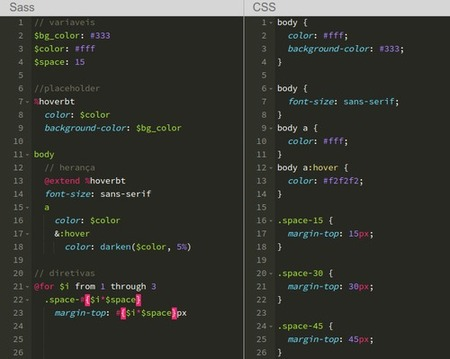
\includegraphics[scale=0.9]{sass.jpg}
            \caption{\small Compilação de um arquivo sass para css}
            \label{cap:sass}
        \end{figure}


    \section{Uglify\label{sec:uglify}}
        É um modulo que funciona em \emph{NodeJs} responsável pela minificação e compressão de arquivos \emph{Javascript}. Minificação consiste em reduzir o código, deixando-o apenas com o que é necessários para seu funcionamento, sem afetar nenhuma funcionalidade.


    \section{Rsync\label{sec:rsync}}
        \emph{Rsync} é uma ferramente que funciona apenas em sistemas \emph{Unix}, responsável por transferência de arquivos e capaz de sincronizar diretórios tanto locais quanto remotos. O \emph{Rsync} pode transferir arquivo \emph{Local -> Local}, \emph{Local -> Remoto}, \emph{Remoto -> Remoto}, \emph{Remoto -> Local}. Ele trabalha sobre o protocolo SSH e \emph{remote-update}, o que aumenta consideravelmente a velocidade e diminui a quantidade de dados transferidos, pois são trocados entre os servidores somente as diferenças entre dois grupos de arquivos reduzindo, também, o consumo de banda, além de ser muito mais seguro.


    \section{Controle de Versão: Git\label{sec:git}}
        É um sistema de controle de versão distribuído e open source que registra as mudanças feitas em um ou mais arquivos de forma que você possa recuperar versões específicas. Ele nos permite reverter arquivos ou até projetos inteiros para um estado anterior, comparar mudanças feitas com o tempo, ver qual desenvolvedor alterou determinado arquivo que pode estar causando problemas, entender em que ponto do projeto surigu determinada falha no sistema entre outras funcionalidades.

    \section{Github\label{sec:github}}
        \emph{Github} é um repositório online que utiliza o \emph{Git} como controle de versão e armazena diversos projetos, facilitando em processos de instalação e permitindo colaboração de outros desenvolvedores.


    \section{Bootstrap\label{sec:bootstrap}}
        É um framework de front-end que tem o objetivo de facilitar o desenvolvimento de interfaces para web. Contém uma coleção de vários elementos e funções personalizáveis para projetos da web, empacotados previamente em uma única ferramenta. Por se tratar de um software livre, todos os seus elementos são personalizaveis e utilizam uma combinação de HTML, CSS e Javascript.

    \section{Javascript\label{sec:javascript}}
        É uma linguagem de programação \emph{client-side} utilizada para controlar \emph{HTML} e \emph{CSS} manipulando comportamentos e elementos de páginas web.


    \section{Jquery\label{sec:jquery}}
        É uma biblioteca que tem como objetivo simplificar tarefas complexas da programação em \emph{Javascript}. Sua intenção é que fazer com que o desenvolvedor codifique menos porém tenha o mesmo, ou um melhor resultado sobre determinada ação.

        Entre as suas características principais, a biblioteca jQuery contém:

        \begin{itemize}
            \item Manipulação do HTML/DOM;
            \item Manipulação CSS;
            \item Métodos de eventos HTML;
            \item Efeitos e animações;
            \item (\emph{AJAX}) Ferramenta Jquery para trocar de informações com servidor sem precisar atualizar a página web atual;
            \item Entre outras funcionalidades genéricas.
        \end{itemize}


% Capitulo 4
\chapter{Estrutura e funcionamento\label{cap:detalhamento-projeto}}

    \section{Processo de instalação\label{sec:processo-instalacao}}
        O \emph{Framework Lothus\{PHP\}} permite ao desenvolvedor a possibilidade de escolha entre dois níves de aplicação. O primeiro nível permite a instalação do \emph{Framework} da forma mais simples, instalando utilitário focados em um desenvolvimento direcionado ao backend do projeto, integrando facilidade a troca de informações com o banco de dados, desenvolvimento através do MVC, URLs amigáves e sistemas de templates.

        Essa instalação é feita através do repositório remoto \emph{Github}, que se encontra no seguinte endereço online:

        \emph{https://github.com/guilouro/Lothus-PHP}

        O Github permite duas formas de download de um projeto: fazendo o downloand de um arquivo comprimido em .zip diretamente do site ou utilizando um sistema de versionamento de arquivos para fazer o clone do mesmo. Neste projetos iremos usar o \emph{Git} como sistema de versionamento. Para fazer o clone utilizando o git executamos a seguinte linha de comando no terminal Unix ou cmd Windows:

        \textbf{\$ git clone https://github.com/guilouro/Lothus-PHP.git}

        Ao executar essa linha de comando, uma nova pasta será criada com o nome de Lothus-PHP. Dentro desta nova pasta estará todo o projeto para iniciar o desenvolvimento utilizando o \emph{Framework Lothus\{PHP\}}. O próximo capítulo será responsável pela apresentação das pastas existentes dentro do projeto.



    \section{Estrutura de pastas e arquivos\label{sec:estrutura-pastas}}
        Neste capítulo será apresentado a estrutura de pastas do \emph{Framework Lothus\{PHP\}} juntamente com o processo de criação e funcionamento de cada etapa.

        Ao clonar o projeto utilizando o git, como visto no capítulo anterior, será gerada uma estrutura de pastas dentro da pasta Lothus-PHP.

        \begin{figure}[!htb]
            \centering
            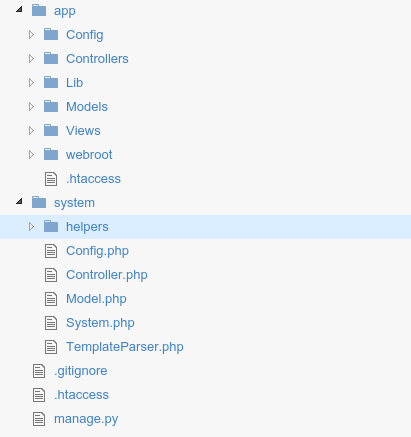
\includegraphics[scale=0.8]{pastas.jpg}
            \caption{\small Estrutura do projeto}
            \label{cap:sass}
        \end{figure}

        Neste primeiro momento já ocorre uma pequena divisão do projeto onde a pasta \emph{app} é responsável por gerenciar a aplicação e a pasta \emph{system} responsável pelo \emph{core}, ou seja, gerenciamento interno do framework. Em sua raiz existe, além dessas duas pastas, três importantes arquivos para o projeto, que são:

        \begin{itemize}
            \item \textbf{.gitignore}: Um arquivo que faz parte da configuração do git e é responsável por guardar, linha por linha, todos os arquivos ou pastas serão ignorados pelo git no momento de fazer o versionamento do projeto. Isso evita o acumulo de arquivos desnecessários, que são gerados automaticamente, no pacote de instalação do Framework.

            \item \textbf{.htaccess}: Arquivo que é lido antes do index.php e tem a responsabilidade de criar a rota inicial do projeto, fazendo o direcionamento para o arquivo correto na inicialização do sistema.

            \begin{figure}[!htb]
                \centering
                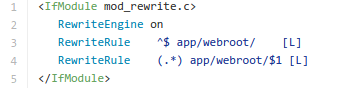
\includegraphics[scale=0.8]{htaccess1.jpg}
                \caption{\small Estrutura do htaccess na raiz do projeto}
                \label{cap:sass}
            \end{figure}

            \item \textbf{manage.py}: Trata-se de um script de linha de comando capaz de gerar novos arquivos baseados na arquitetura de funcionamento do \emph{Framework}. A imagem abaixo ilustra o uso básico da ferramenta.

            \begin{figure}[!htb]
                \centering
                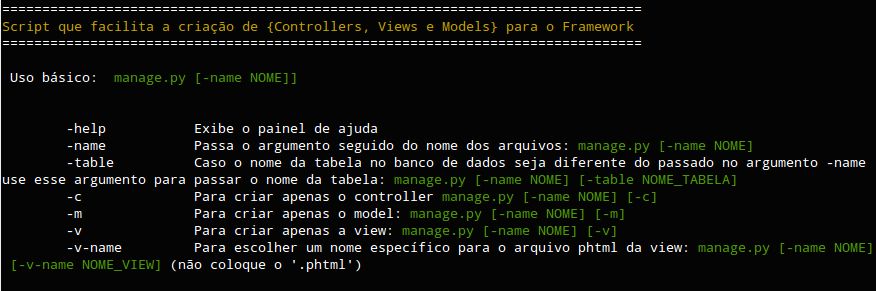
\includegraphics[scale=0.5]{manage.jpg}
                \caption{\small Regras para uso básico do manage.py}
                \label{cap:sass}
            \end{figure}


        \end{itemize}

    \section{Sistema\label{sec:system-core}}

        O Framework recebe um primeiro nível de divisão no processo de criação do mesmo, que é a divisão do Sistema da Aplicação. O sistema fica todo centralizado na pasta \emph{system}, e é onde contém o motor do \emph{Framework}, nele estão todas as classes responsáveis pelas regras de funcionamento do projeto, tanto nas requisições HTTP, passando por padronização de Controllers, Views até chegar ao relacionamento com o banco de dados. Todas essas funcionalidades estão divididas entre classes e arquivos que serão detalhados ao longo deste capítulo.

    \begin{figure}[!htb]
        \centering
        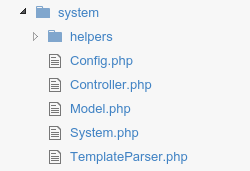
\includegraphics[scale=0.6]{system-path.jpg}
        \caption{\small Estrutura interna da pasta system}
        \label{cap:sass}
    \end{figure}



        \subsection{Config\label{sub:system-config}}

            A Classe \emph{Config} é responsável pela configuração inicial de qualquer projeto que faz uso do \emph{Lothus\{PHP\}}. Ela tem a responsabilidade de definir qual \emph{View} será iniciada ao acessar o link do sistema e também se responsabiliza em definir se será exibido ou não um \emph{debug} para o desenvolvedor.

            \emph{}

            O arquivo \emph{Config.php} possui a seguinte estrutura:

            \emph{}

\begin{lstlisting}
class Config {
    public  $_Index = "home";
    private $error = TRUE;

    protected function ERROR($pag){}
}
\end{lstlisting}


        \begin{itemize}
            \item\textbf{\$\_Index}: É uma variável \textbf{pública} que recebe, como string, o nome do \emph{Controller} padrão a ser requisitado pelo sistema no caso de a URL não ter, explicitamente, este valor.

            \item\textbf{\$error}: Trata-se de uma \textbf{privada} váriavel booleana, que funciona como uma chave para exibir um erro para o desenvolvedor ou direcionar o usuário para uma página 404, no momento em que for acessada alguma página inexistente. No caso de \textbf{\$error = TRUE} será exibido uma mensagem de alerta ao desenvolvedor sobre alguma falha nos padrões do \emph{Framework}. Caso \textbf{\$error = FALSE} o usuário será redirecionado para uma página de \emph{erro 404}

            \item\textbf{ERROR(\$pag)}: É um método protegido, que recebe como parâmetro o nome da página que não foi encontrada no sistema. Sua funcionalidade é, inicialmente, verificar se a variável \textbf{\$error} é \textbf{TRUE} \emph{(Verdadeiro)} ou \textbf{FALSE} \emph{(False)}, para posteriormente, direcionar o usuário para a página de erro padrão do sistema ou exibir uma mensagem dizendo se o erro foi causado pela falta de um \emph{Controller} ou de uma \emph{Action} para o sistema.
        \end{itemize}

        \emph{}

        \emph{}

        A lógica de programação aplicada a este método é a seguinte:

        \emph{}

\begin{lstlisting}
protected function ERROR($pag) {
    if($this->error) {
        /* Erro em Controller ou Action */
    } else {
        /* Redirecionamento */
    }
}
\end{lstlisting}


        \subsection{System\label{sub:system-sis}}

            O projeto é iniciado com a primeira chamada sendo referenciada à classe \emph{System} que tem como herança os métodos e atributos, que não são privados, da classe \emph{Config}. Sua principal funcionalidade é interpretar o padrão de URL criado para o Framework e fazer a separação para a camada correta de Controllers e actions com seus respectivos parâmetros, quando houver.

            O \emph{Lothus\{PHP\}} usa um padrão de url denominado \textbf{url amigável}, que facilita tanto a leitura dos mecanismos de buscas quanto a leitura do próprio usuário, além de padronizar todos os projetos desenvolvidos pelo \emph{Framework}.

            A URL segue o seguinte padrão:

            \emph{http://urldosite.com.br/\{Controller\}/\{Action\}/\{n-parametros\}}

            \begin{itemize}
                \item\textbf{Controller:} Classe controller referente à página acessada
                \item\textbf{Action:} Método existente nessa mesma classe
                \item\textbf{n-parametros:} Será passado como argumento para a o método desta mesma classe controller.
            \end{itemize}

            Todos esses itens serão abordados corretamento no momento em que for descrito o funcionamento das classes de Aplicação do projeto.

            Pode se explicar que a classe system, ao ser invocada, recebe a URL via GET e através de alguns métodos essa URL é desmembrada, as variáveis da classe são definidas e por fim o projeto é inicia, como demostrada na estrutura da classe logo abaixo.

\begin{lstlisting}
class System extends Config {

    public $_url;
    private $_explode;
    public  $_controller;
    public  $_action;
    public  $_params;

    public function init(){}
    private function setUrl(){}
    private function setExplode(){}
    private function setSlug($w){}
    private function setController(){}
    private function setAction(){}
    public function setParams(){}
    public function setGets(){}
    public function run(){}
}
\end{lstlisting}

            A classe possui alguns atributos responsáveis por guardar determinadas informações a serem utilizadas em diversas etapas de sua leitura. Esses atributos tem suas responsabilidades descritas abaixo.

            \begin{itemize}
                \item\textbf{\$\_url}: Atributo público que receberá a url atual como string.
                \item\textbf{\$\_explode}: É um vetor privado que receberá, em cada uma de sua posição, uma parte da URL que se utiliza da \emph{"/"} como regra de separação.
                \item\textbf{\$\_controller}: Atributo público que guardará o nome do Controller a ser usado.
                \item\textbf{\$\_action}: Atributo público que guardará o nome da Action a ser usada.
                \item\textbf{\$\_params}: Vetor público que guardará todos os parâmetros passados pela URL.
            \end{itemize}

            Esses valores são atribuídos através dos métodos que além de atribuir fazem uso dessas mesmas variáves da classe, como descrito nos elementos de cada método abaixo.
.
            \begin{itemize}

                \item\textbf{init()}: Primeiro método a ser chamado, explicitamente, pela classe e responsável por fazer a chamada de todos os métodos que fazem as atribuíções a todas as variáves dessa classe.
\begin{lstlisting}
public function init() {
    $this->setUrl();
    $this->setExplode();
    $this->setController();
    $this->setAction();
    $this->setParams();
    $this->setGets();
}
\end{lstlisting}

                \item\textbf{setUrl()}: Responsável por atribuir a string da URL atual para a variável \textbf{\$\_url}. Caso a URL passada não tenha, explicitamente um controller e uma action, será atribuído o valor da variável \textbf{\$\_Index}, que é uma herança da classe Config, juntamente com a action padrão \textbf{index\_action}.
\begin{lstlisting}
private function setUrl() {
    $this->_url = (isset($_GET['url']) ? $_GET['url']  :
        $this->_Index . "/index_action" );
}
\end{lstlisting}

                \item\textbf{setExplode()}: Método que atribui ao array\emph{(Vetor)} \textbf{\$\_explode} os valores passados para a variável \textbf{\$\_url} e delimitados pela barra\emph("/").

\begin{lstlisting}
private function setExplode(){
    $this->_explode = explode("/", $this->_url);
}
\end{lstlisting}

                \item\textbf{setController()}: Define qual controller será usadado para a requisição atual, através do primeiro índice do vetor \textbf{\$\_explode}

\begin{lstlisting}
private function setController(){
    $this->_controller = $this -> setSlug($this -> _explode[0]);
}
\end{lstlisting}

                \item\textbf{setAction()}: Define qual action será usadado para a requisição atual, através do segundo índice do vetor \textbf{\$\_explode}. Caso não exista, será atribuído o valor \textbf{"index\_action"}.

\begin{lstlisting}
private function setAction(){
    $this->_action = $this -> setSlug(
        !isset($this->_explode[1]) ||
        $this->_explode[1] == null ||
        $this->_explode[1] == 'index' ? 'index_action' :
        $this->_explode[1]);
}
\end{lstlisting}

                \item\textbf{setParams()}: Responsável por criar o vetor para todos os parâmetros passados pela URL atual. Parâmetros esses que são definidos por todos o valores passados além do controller e action na string da URL.

\begin{lstlisting}
public function setParams(){
    unset($this->_explode[0], $this->_explode[1]);
    if( end( $this->_explode ) == null )
        array_pop($this->_explode);
    $this->_params = $this->_explode;
}
\end{lstlisting}

                \item\textbf{setGets()}: Verifica a aparição da requisição GET no HTTP da página atual e define o vetor \textbf{\$\_GET} do PHP com seus respectivos valores.

\begin{lstlisting}
public function setGets(){
    $url = $_SERVER['REQUEST_URI'];
    $url = explode("?", $url);
    if(isset($url[1])) {
        $urlParams = explode("&", $url[1]);
        foreach ($urlParams as $g) {
            $get = explode("=", $g);
            $_GET[$get[0]] = $get[1];
        }
    }
}
\end{lstlisting}

                \item\textbf{setSlug(\$w)}: É responsável por verificar se o item \textbf{\$w} possui duas ou mais palavras separadas por ífem. Caso exista, esse método retira os ífens e transforma todas essas palavras em apenas uma no modo \emph{CamelCase}.

\begin{lstlisting}
private function setSlug($w){
    $arr = explode("-", $w);
    for ($i=1; $i < count($arr); $i++) {
        $arr[$i] = ucfirst($arr[$i]);
    }
    $slug = implode("", $arr);
    return $slug;
}
\end{lstlisting}

                \item\textbf{run()}: É o método responsável por carregar o controller e a action com todos os parâmetros, caso eles existam. Se algum desses objetos não forem encontrado, o método \textbf{\$ERROR}, herdado da classe \emph{Config}, é chamado para exibir a mensagem adequada ao usuário.

            \end{itemize}



        \subsection{Helpers\label{sub:system-helper}}
            São classes que auxiliam o desenvolvedor no andamento do projeto, podendo ou não ser utilizadas em determinadas aplicações. O \emph{Framework} vem com algumas classes em sua instalação, podendo ser adicionadas outras se o desenvolvedor sentir necessidade. As classes se encontram dentro da pasta \textbf{helpers} e segue um padrão de nomenclatura que é o nome da classe acompanhada da palavra \emph{Helper}. Para uma classe chamada \textbf{Email} teria que ter a seguinte nomenclatura: \textbf{EmailHelper}.

            O projeto acompanha algumas classes que serão descritas logo abaixo:

            \begin{itemize}
                \item\textbf{AuthHelper}: Auxilia na autenticação de usuários para projetos que possuem áreas restritas. Ela se responsabiliza em fazer o login do usuário no sistema de forma segura, comparando a senha digitada com a que possui no banco de dados através da criptografia \textbf{sha512} e iniciando uma sessão para o usuário. Possui um métdo de logout, onde finaliza uma sessão com o usuário e o desconecta da área restrita do sistema. Além de possuir métodos que ajudam no controle de páginas protegidas, fazendo a verificação da permissão cada vez que o usuário tenta acessar a mesma.

                \item\textbf{EmailHelper}: Classe auxiliadora para envio de emails. Extende à classe \emph{PHPMailer} e trabalha como uma facilidadora para esta, que é uma ferramenta avançada para envio de emails em \emph{php}.

                \item\textbf{ImageHelper}: Esta é uma classe para otimização e salvamento de imagens nos projetos. Ela pode trabalhar tanto com imagens enviadas por um formulário quanto imagens provenientes de algum link da internet. Sua estrutura é formada apenas por um construtor e mais 3 métodos públicos. Ós métodos \textbf{ResizeByUrl} e \textbf{ResizeByUpload} salvam o arquivo de imagem na pasta especificada através do construtor da classe e retornam o nome gerado para o arquivo pelo método \textbf{Rename}. Esse nome é gerado para evitar a criação de imagens caractéres especiais em seu nome evitando inclusive, sobrescrever imagens com o mesmo nome. A classe obedece a seguinte estrutura descrita abaixo:

\begin{lstlisting}
class ImageHelper {

    private $_ALTURA_PADRAO;
    private $_pasta;

    /*
     * Metodo construtor
     * @param $pasta = Nome da pasta para upload
     * @param $altura_padrao = Definir uma altura padrão para os arquivos
     */
    function __construct($pasta, $altura_padrao = null) { }

    /*
     * Metodo ResizeByUrl
     * Salva uma imagem a partir de um link
     * @param $url = Url da imagem a ser salva
     * @param $altura = Definir uma altura para a imagem atual, caso seja diferente da altura padrão
     */
    public function ResizeByUrl($url, $altura = null) { }

    /*
     * Metodo ResizeByUrl
     * Salva uma imagem a partir de upload
     * @param $imagem = ex: $_FILES['imagem']
     * @param $altura = Definir uma altura para a imagem atual, caso seja diferente da altura padrão
     */
    public function ResizeByUpload($imagem, $altura = null) { }

    /*
     * Metodo Rename
     * Remove acentos, espaços e caracteres especiais e cria um nome aleatório.
     * @param $string = string a ser limpa
     */
    public function Rename( $string ) { }
}
\end{lstlisting}

            \item\textbf{PaginationHelper}: Classe capaz de dividir um conteúdo vindo do banco de dados em diversas páginas através de uma paginação. A classe permite, ao ser instanciada, receber o nome da tabela no banco de dados que será feita a consulta. Essa consulta possibilita ao desenvolvedor escolher quantos itens serão exibidos por páginas e a ordem de exibiçao. Além dessa exibição ela fornece alguns métodos auxiliares onde se pode ter o retorno da página ou url atual. A classe possui uma estrutura bem simples como mostrada abaixo.

\begin{lstlisting}
class PaginationHelper
{
    private $_model;
    private $_limite;
    private $_paginaAtual;
    private $_inicio;
    private $_total_registros;

    /**
     * Classe para paginação
     * @param String $tabela tabela no banco de dados para a consulta
     */
    function __construct( $tabela ) { }

    /**
     * Pega a quantidade total de páginas de acordo com a lista
     * @return int retorna a quantidade de páginas
     */
    public function totalPaginas() { }

    /**
     * Responsável por fazer a consulta limitada
     * para a paginação e definição de alguns atributos
     * @param  Array $arr parâmetros SQL. 'where' , 'orderby'
     * @return Array      retorna a consulta limitada
     */
    public function consulta(Array $arr = null) { }

    /**
     * Retorna a página atual captura
     * @return int
     */
    public function getPaginaAtual() { }

    /**
     * Gera url atual
     * @return string retorna a url até a parte da pagina
     */
    public function getUrl() { }

    /**
     * Cria a view para exibição da paginação
     * @param  string $classe define a classe da div que engloba a paginação
     * @return string
     */
    public function view($classe = "pagination pagination-centered") { }
}
\end{lstlisting}

            Ao fazer a chamado do método \textbf{view()} no template do sistema, um componente de paginação é criado de acordo com a quantidade de páginas existente na sessão atual. Esse método, por padrão, cria o componente com uma classe de \emph{css} referente ao framework \emph{Bootstrap}. Com isso o componente passa a ter uma formatação adequada para uma paginação.

            \begin{figure}[!htb]
                \centering
                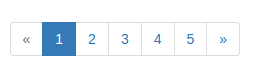
\includegraphics[scale=1]{paginacao.png}
                \caption{\small Componente de paginação criado por PaginatioHelper}
                \label{cap:paginaca}
            \end{figure}


            \item\textbf{RedirectHelper}: Simples classe que fornece a possibilidade de trabalhar com redirecionamento dentro do projeto. Possui métodos para retorno de url, \emph{Controller} atual e \emph{Action} atual. Seu métodos principais são os de redirecionamento, tomando como base o \emph{controller}, a \emph{action} ou ambos como ponto de destino para este redirecionamento. A classe e seus principais métodos podem ser vistas no modelo abaixo:


\begin{lstlisting}
class RedirectHelper {
    ...

    /**
     * Retorna o controller atual
     * @return (String)
     */
    public function getCurrentController() { }

    /**
     * Retorna a action atual
     * @return (String)
     */
    public function getCurrentAction() { }

    /**
     * Redireciona para o controller especificado
     * @param  (String) nome do controller
     * @return void
     */
    public function goToController( $controller ) { }

    /**
     * Redireciona para a action especificada
     * @param  (String) nome da string
     * @param  (boolean) para usar parâmetro global
     * @return void
     */
    public function goToAction( $action, $paramsGlobal = FALSE ) { }

    /**
     * Redireciona para controller e action especificada
     * @param  (String) nome controller
     * @param  (String) nome action
     * @return void
     */
    public function goToControllerAction( $controller, $action ) { }

    ...

}
\end{lstlisting}

            \end{itemize}



        \subsection{Controller\label{sub:system-controller}}
            Essa classe recebe a \emph{System} como herança e possui, inicialmente, dois métodos e um atributo. Sua função é guardar o template que será usado e compitar a view para o sistema. A estrutura da classa está descrita abaixo.


\begin{lstlisting}
class Controller extends System {

    public $_layout = 'default';

    protected function view($nome_pagina, $vars = null) { }

    public function init() { }
}
\end{lstlisting}

            \begin{itemize}
                \item\textbf{\$\_layout}: Atributo público para definir o template base da página a ser carregada.
                \item\textbf{view(\$nome\_pagina, \$vars \= null)}: Método responsável por atribuir o template da view ao template base, e recebe como primeiro parâmetro \emph{(\$nome\_pagina)} o nome do arquivo do template a ser utilizado. O Método possui um segundo parâmetro \emph{(\$vars)} opcional, que é capaz de receber um vetor e distribuí-lo em variáveis para ser utilizada no template carregado.

                \item\textbf{init()}: É o primeiro método a ser chamado no momento da criação do Controller. Ele pode ser ou não implementado dentro de cada controller criado e é o primeiro método a ser executado sempre que carrega uma página.
            \end{itemize}


        % \subsection{Url amigável e o padrão MVC\label{sub:url-amigavel}}

        \subsection{Model\label{sub:system-model}}
            Classe responsável por fazer a comunicação entre aplicação e banco de dados. Utizando, como padrão, o módulo nativo do php chamado \emph{PDO}. Esta classe segue a seguinte estrutura descrita abaixo.


\begin{lstlisting}
class Model {
    protected $db;
    public    $_tabela;
    public    $_fk;

    public function __construct()  { }

    public function insert( Array $dados, $debug = FALSE ) { }

    public function read( $where = null , $limit = null ,
        $offset = null , $orderby = null, $debug = FALSE ) { }

    public function readLine( $where = null , $limit = null ,
        $offset = null , $orderby = null, $debug = FALSE ) { }

    public function update( Array $dados, $where, $debug = FALSE ) { }

    public function delete( $where ) { }

    public function consulta($sql, $debug = FALSE) { }

    public function consultaLinha ( $sql , $debug = FALSE ) { }

    public function consultaValor ( $sql , $debug = FALSE ) { }

    public function populateFK() { }

}
\end{lstlisting}

            \begin{itemize}
                \item\textbf{\$db}: Atributo protegido que se torna uma instância da classe \emph{PDO}, capaz de fazer o processo de envio e recebimento de dados entre aplicação e banco de dados. Este objeto é instanciado através do construtor da classe.

                \item\textbf{\$\_tabela}: Atributo público que guarda uma \emph{string} como o nome da tabela, existente no banco de dados, que será manipulada pela classe.

                \item\textbf{\$\_fk}: Atributo que recebe um vetor, no caso de existeir relações entre tabelas, ligadas com chave estrangeira.

                \item\textbf{insert(Array \$dados, \$debug\=FALSE)}: Método público, responsável por fazer a inserção de novos dados na tabela que está especificada na classe. O metodo \emph{insert} recebe como parâmetro um vetor, denominado \textbf{\$dados}, com os dados a serem inseridos. Este vetor, por padrão precisa conter no mínimo uma chave e um valor, onde a chave será o nome da coluna e o valor será o conteúdo desta coluna a ser inserido no banco de dados. O retorno deste método é o \emph{Id} da linha inserida caso a ação seja bem sucedida, do contrário retornará um valor nulo. O método permite um segundo parâmetro, opcional, chamado textbf{\$debug}. Debug aceita valores \emph{booleanos} onde, se receber \textbf{true} ele imprime na tela a string completa que faz a interação naquele momento com o banco de dados, no caso de \textbf{false} ele não faz nada. Por padrão \textbf{\$debud} é iniciado como falso.

                \item\textbf{read(\$where\=null, \$limit\=null, \$offset\=null, \$orderby\=null, \$debug\=FALSE)}: Método público, responsável pela consulta direcionada à tabela especificada na classe. Este método fornece ao desenvolvedor a possibilidade de passar alguns parâmetros, responsáveis pela filtradem dos dados retornados. A passagem de parâmetro é opcional e possui nomenclaturas intuitivas que auxiliam no entendimento das funcionalidades. Por padrão o método \emph{read()}, sem passar parâmetro algum, retorna um vetor com dados relacionado a uma consulta completa e sem filtros da tabela especificada. O restorno pode ser filtrado definindo os parâmentros do método.
                \begin{itemize}
                    \item\textbf{\$where}: Condição a ser tratada pela clausula \emph{WHERE} do mysql na consulta solicitada.
                    \item\textbf{\$limit}: Responsável por determinar o ponto final, através da quantidade de linhas retornadas.
                    \item\textbf{\$offset}: Responsável por determinar o ponto inicial, através da quantidade de linhas retornadas.
                    \item\textbf{\$orderby}: Nome da coluna em que a consulta usa como base para ordenação do resultado.
                    \item\textbf{\$debug}: Imprime na tela a string completa que faz a interação naquele momento com o banco de dados.
                \end{itemize}

                \item\textbf{readLine(\$where\=null, \$limit\=null, \$offset\=null , \$orderby\=null, \$debug\=FALSE)}: Tem a mesma caracterísca do método \emph{read()}, porém o seu retorno é de um vetor com apenas um indice baseado em uma consulta de uma linha do banco de dados.

                \item\textbf{update(Array \$dados, \$where, \$debug\=FALSE)}: Atualiza os dados em determinada linha de uma tabela, utilizado o \emph{UPDATE} do mysql. O método possui a necessidade de passagem de dois parâmetros obrigatórios e da a opção de um terceiro parâmetro não obrigatório, são eles:
                \end{itemize}
                    \item\textbf{\$dados}: Parâmetro obrigatório que possui um vetor com os dados a serem atualizados no banco de dados.
                    \item\textbf{\$where}: Parâmetro obrigatório com a condição a ser utilizada pelo \emph{WHERE} do mysql, com a responsabilidade de tratar em quais linhas da tabela serão feitas as subistituições solicitadas.
                    \item\textbf{\$debug}: Imprime na tela a string completa que faz a interação naquele momento com o banco de dados.
                \begin{itemize}

                \item\textbf{delete(\$where)}: Exclui uma linha do banco de dados referente à condição passada pelo parâmentro \textbf{\$where}

                \item\textbf{consulta(\$sql, \$debug\=FALSE)}: Este método permite ao desenvolvedor passar uma string completa de sql para retornar um conjunto de linhas específicos a essa consulta. O método recebe as regras da consulta, faz a busca no banco de dados e retora um vetor com todas as linhas da tabela referente à consulta. Esse método não utiliza a variável \$\_tabela como referência ao banco de dados e aceita dois parâmetros, que são os seguintes:
                \end{itemize}
                    \item\textbf{\$sql}: Parâmetro obrigatório que recebe a string completa de consulta ao banco de dados.
                    \item\textbf{\$debug}: Imprime na tela a string completa que faz a interação naquele momento com o banco de dados.
                \begin{itemize}

                \item\textbf{consultaLinha(\$sql, \$debug\=FALSE)}: Este método permite ao desenvolvedor passar uma string completa de sql para retornar apenas uma linha referente a essa consulta. O método recebe as regras da consulta, faz a busca no banco de dados e retora um vetor uma linha da consulta efetuada. Esse método não utiliza a variável \$\_tabela como referência ao banco de dados e aceita dois parâmetros, que são os seguintes:
                \end{itemize}
                    \item\textbf{\$sql}: Parâmetro obrigatório que recebe a string completa de consulta ao banco de dados.
                    \item\textbf{\$debug}: Imprime na tela a string completa que faz a interação naquele momento com o banco de dados.
                \begin{itemize}

                \item\textbf{consultaValor(\$sql, \$debug\=FALSE)}: Este método permite ao desenvolvedor passar uma string completa de sql para retornar apenas um valor referente a essa consulta. O método recebe as regras da consulta, faz a busca no banco de dados e retora um único valor da consulta efetuada. Esse método não utiliza a variável \$\_tabela como referência ao banco de dados e aceita dois parâmetros, que são os seguintes:
                \end{itemize}
                    \item\textbf{\$sql}: Parâmetro obrigatório que recebe a string completa de consulta ao banco de dados.
                    \item\textbf{\$debug}: Imprime na tela a string completa que faz a interação naquele momento com o banco de dados.
                \begin{itemize}

                \item\textbf{populateFK()}: Caso a variável \textbf{\$\_fk} possua um vetor como valor, este método é capaz de percorrer cada valor, executar o método \emph{read()} referente a cada tabela e popular o retorno para uma variável como mesmo nome da tabela do banco de dados.

            \end{itemize}

        \subsection{Template\label{sub:system-template}}

            O \emph{Framework Lothus\{PHP\}} possui uma forma de se trabalhar com templates e esse controle é feito através da classe \emph{TemplateParser}. A classe herda os valores e métodos da classe \emph{System}, o que permite a manipulação e utilização de alguns dados. Os templates ficam localizados dentro da pasta \empt{app\\Views\\Layouts} e por padrão o template principal é o \emph{default\.phtml}. O \emph{Framework} permite trabalhar com diversos templates, para isso existe algumas regras a serem seguidas. Primeiramente precisa ser criado um arquivo como o nome do template dentro da pasta \empt{app\\Views\\Layouts} do projeto atual, por exemplo \textbf{novo\_template.phtml}. Em seguinda é necessário inserir a tag \emph{\{conteudo\}} no local onde serão exibidas as views dependentes deste template. E finalmente dizer em quais actions do sistema farão uso desse template definindo a variábel de layout com o valor do novo template \emph{\$this->\_layout = \'novo\_template\'}. Esta variável é definida dentro do método que será responsável pela action da página em questão.

            A funcionamento dos templates é, verificar o template padrão a ser usado, através da variável \emph{\$\_layout}, que pertence à classe \emph{Controller}, que por padrão é \emph{\'default\'}, em seguinda é feito a busca da tag \emph{\{conteudo\}} dentro deste template e esta tag é, por fim, substituída pela view que será exibida.


    \section{Aplicação\label{sec:app}}

        O Framework recebe um segundo nível de divisão no processo de criação do mesmo, que é a parte da App, onde será construído toda a aplicação. A aplicação fica toda centralizada na pasta \emph{app}, que é onde contem a divisão \emph{MVC} da aplicação. Todas essas funcionalidades estão divididas entre classes e arquivos que serão detalhados ao longo deste capítulo.

    \begin{figure}[!htb]
        \centering
        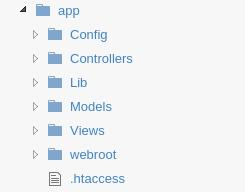
\includegraphics[scale=0.6]{app-path.jpg}
        \caption{\small Estrutura interna da pasta app}
        \label{cap:sass}
    \end{figure}

        \subsection{Config\label{sec:app-config}}

        \subsection{Model\label{sec:app-model}}

        \subsection{View\label{sec:app-view}}

        \subsection{Controller\label{sec:app-controller}}

        \subsection{Lib\label{sec:app-lib}}

        \subsection{webroot\label{sec:app-lib}}


        \subsection{Controller\label{sec:app-controller}}


    \section{Divisão Backend - frontend\label{sec:back-front}}


        \subsection{Comandos do Grunt\label{sub:comandos-grunt}}


% Capitulo 4
\chapter{Experimento com Framework existente\label{cap:experimento}}

    \section{Cake PHP\label{sec:cake-php}}
        \subsection{Descricao da ferramenta\label{sub:descricao-cake}}

            O CakePHP é um projeto de código aberto mantido por uma comunidade bastante ativa de desenvolvedores PHP. Possui uma estrutura extensível para desenvolvimento, manutenção e implantação de aplicativos. Utiliza o padrão de projeto MVC\emph{(Model-View-Controller)} e ORM\emph{(Object-relational mappring)} com os paradigmas das convenções sobre configurações.


        \subsection{Objetivo\label{sub:objetivo-cake}}

            CakePHP tem como objetivo principal a simplificação do processo de desenvolvimento e construção de aplicações web, utilizando um núcleo onde organiza o banco de dados e alguns recursos que reduzem a codificação pelo desenvolvedor. Alguns desses recursos são a validação embutida, ACLs \emph{(lista de controle de acesso)}, segurança, manipulação de sessão e cache de Views e sanitização de dados.


        \subsection{Características\label{sub:caracteristicas-cake}}
            \begin{itemize}
                \item Ativo e com comunidade amigável
                \item Compatível com PHP5
                \item Geração de CRUD (\emph{Create, Read, Update and Delete, ou Criar, Ler, Atualizar e Excluir})
                \item Funciona em qualquer subdiretório web, com poucas configurações no apache
                \item Utiliza templates
            \end{itemize}


%===================================================================================
%\backmatter
%===================================================================================

%\bibliography{monografia}{}
%\bibliographystyle{abnt-alf}

% OUTRA FORMA DE CRIAR A BIBLIOGRAFIA:

\begin{thebibliography}{9}

    \bibitem{unesco}Relatório Unesco Sobre Ciência. Disponível em: \url{http://unesdoc.unesco.org/images/0018/001898/189883por.pdf}.
    Acesso em: 26 fev. 2015.

\end{thebibliography}


\anexo
\end{document}